\documentclass[a4paper, 11pt]{article}
\usepackage[utf8]{inputenc}
\usepackage{graphicx,wrapfig,subfigure,amsmath,amssymb,epsfig,bm}
\usepackage{listings,textcomp,color,geometry,siunitx}
\geometry{hmargin=2cm, vmargin=2cm}

\def\Box{\mathord{\dalemb{7.9}{8}\hbox{\hskip1pt}}}
\def\dalemb#1#2{{\vbox{\hrule height.#2pt
        \hbox{\vrule width.#2pt height#1pt \kern#1pt \vrule width.#2pt}
        \hrule height.#2pt}}}

\def\eop{\mathcal{E}}
\def\bop{\mathcal{B}}
\def\ba{\begin{eqnarray}}
\def\ea{\end{eqnarray}}
\def\be{\begin{equation}}
\def\ee{\end{equation}}
\def\tr{{\rm tr}}
\def\Var{{\rm Var}}
\def\gtorder{\mathrel{\raise.3ex\hbox{$>$}\mkern-14mu
             \lower0.6ex\hbox{$\sim$}}}
\def\ltorder{\mathrel{\raise.3ex\hbox{$<$}\mkern-14mu
             \lower0.6ex\hbox{$\sim$}}}

\def\bb{{\mathfrak b}}
\newcommand{\ellb }{\boldsymbol{\ell }}

% Personal colors defined here
\newcommand{\skn}[1]{{\color{red}#1}}
\newcommand{\TIB}[1]{{\color{blue}#1}}
\newcommand{\assume}[1]{{\bf#1}}

\begin{document}

\title{\textbf{ACTPol Cookbook}}
\author{The ACTPol collaboration}
\maketitle

The goal of this document is not to be exhaustive, not to be complete, not
to be free of typos, not to be circulated outside the AdvACT collaboration.
It is supposed to be a living document.  Choose your color for
editing/asking clarification in other people sections: \skn{Sigurd}, \TIB{Thibaut}.

\section{TOD cut and calibration}

The cuts and calibration pipelines are using the moby2 framework. We can divide it in three steps:
\begin{itemize}
\item data selection,
\item relative calibration of detectors and TODs to physical units,
\item absolute calibration to CMB temperature.
\end{itemize}
The first two steps are performed at the individual TOD level, using detector properties measurements (IV, Bias Step, dark detectors, thermometers) and sky signal, mostly dominated by the atmosphere. The last step is performed a posteriori using planet measurements for the whole season, planet and atmosphere models, and beam characterization.



\subsection{Data selection (\emph{cuts})}
The general philosophy of the data selection is to characterize each detector behavior in two different frequency bands. At the lowest frequencies, we expect the dominant signal to be the atmosphere, and thus the detectors to show a good correlation between them (at first order the atmosphere is common to the whole array). It also provides a relative calibrator. At the highest frequencies, the signal is dominated by the detector noise, expected to be white.

\subsubsection{Data description}
\subsubsection{Pre-processing}
A few steps of pre-processing are applied before running the core of the cuts pipeline. They are detailed here:
\begin{itemize}
	\item trim the TOD: some processes tend to warm up the focal plane, requiring a security buffer time before the temperature equilibrium is reached again. It is the case for IV curves and re-biasing for example. We thus discard all samples too close to these events. The buffer times are defined in the input parameter file as \emph{IV\_wait} and \emph{rebias\_wait}; we have been using respectively $220$s and $25$s after IV and re-biasing events.
	\item substract \emph{$A(\chi)$}: if an $A(\chi)$ model is provided in the parameter file, it will be deprojected. It hasn't been used yet as test results were not really convincing.
	\item cut mce frame errors: cut glitches from readout.
	\item cut planets and sources: planets and sources provided in the parameter file will be masked. The mask is a circle around the theoretical position of the planet/source. Radius of the mask and pointing models are needed as inputs and defined in the parameter file. These cuts are stored under \emph{tag\_source} and \emph{tag\_planet}.
	\item cut glitches: timelines are bandpass filtered and glitches are flagged as everything above a threshold defined relatively to the noise level. Parameters of the filter and threshold are defined in the parameter file. This cut (plus the mce frame error) is stored as \emph{tag\_partial}.
	\item remove the mean of the TOD: as the absolute scale of the data is irrelevant, we remove the mean (or median if specified in the parameter file) of each detector timeline.
	\item detrend: a straight line between the first and last sample of the timelines is removed to ensure boundary conditions for the FFT. Lowest frequencies are filtered out later on anyway. \emph{detrend = True} has to be explicitly specified in the parameter file, as it is set to \emph{False} by default.
	\item remove filter gain: if \emph{remove\_filter\_gain = True} is specified in the parameter file, the filter gain will be removed. Default is \emph{False}.
	\item downsample: timelines can be downsampled by a {}factor $2^{n\_downsample}$ where $n\_downsample$ is specified in the parameter file.
	\item find zero detectors: discard detectors that have zero signal.
	\item find jumps: discard detectors that have jumps in the timeline.
	\item calibrate to pW: use the responsivity from Bias Step (or IV) and the flatfield to calibrate the TODs to pW. Responsivity and flatfields to use are defined in the parameter file.
	\item FFT: get the fourier transform of the timestreams.
\end{itemize}

\subsubsection{Low frequency}
\label{subsubsection:lfcuts}
After these pre-processing steps, we perform the low frequency part of the analysis, in which we want to use the atmospheric signal to select live detectors and get a relative calibration for them (see \ref{subsec:relcal}). First we'll describe the procedure and then see a couple of modules that can be applied to the procedure.

\subsubsection*{General procedure}
\begin{itemize}
	\item Select only the low frequency modes of the data ($\sim [0.01,0.1]$Hz).
	\item Compute the norm of the data for each detector.
	\item Compute the full correlation matrix for all detectors.
	\item Pre-select a group of "good" detectors based on this matrix (see below for a description).
	\item Compute the SVD of the pre-selected data.
	\item For each detector, compute the correlation (\emph{corr}) to the main mode (or the two main modes) of the SVD, and the coefficient/gain (\emph{gain}).
	\item Compute the RMS of the data after de-projecting $n$ modes (usually 3) from the full data SVD. We call it Drift Error (\emph{DE}).
\end{itemize}

From this low-frequency analysis, we keep three criteria that are \emph{corr}, \emph{gain} and \emph{DE} that will be used to select valid detectors. An extra criteria  \emph{darkRatio} can be computed if the thermal contamination module (see below) is turned on.


\subsubsection*{Thermal contamination}
Dark detectors can be used to clean the live detectors from contamination. At low frequency, we mostly expect this contamination to be thermal, and it can contribute to the signal to a comparable level as the atmosphere (e.g. at low PWV). If the module is turned on, we take the SVD of the normalized dark detectors in the same frequency range, and de-project the first $n$ modes from the live data. The number of modes to be de-projected as well as other parameters are defined in the parameter file in the \emph{darkModesParams} dictionary.

In the case it is applied, a \emph{darkRatio} criteria is outputted for later selection. It is the ratio of the norm of the data after de-projecting the dark modes and the norm before.

\subsubsection*{Scan Frequency rejection}
If the scan frequency is within the chosen low frequency window, we can mask it using the \emph{cancelSync = True} parameter. It will put to $0$ the data at scan frequency (and its harmonics).

\subsubsection*{Pre-selection of good detectors}
Two methods can be used to pre-select the group of detectors to be used to extract the common mode.
\begin{itemize}
	\item \textbf{median} uses a two iteration selection based on the correlation matrix, throwing away the detectors with an average correlation to the others lower than a threshold that is relatively low at the first iterationand then increased at the second.
	\item \textbf{groups} uses an iterative \emph{friends-of-friends} method to form groups of similar detectors. The main group is then selected. The method relies on a fine tuning of its parameters are defined in the parameter files.
\end{itemize}

\subsubsection*{Multi-frequency analysis}
To avoid step effects due to the choice of the frequency band, we can use $N$ frequency bands using a sliding window and average the results from them. The size of the window, the size and number of steps and the initial frequency are defined in the paramaeter file.

\subsubsection*{Multichroic arrays}
For multichroic arrays, separate frequencies can be treated completely separately using the parameter \emph{separateFreqs}. At the moment we are treating them separately.



\subsubsection{High frequency}
At high frequency, we are interested in the noise properties. We use only the modes of the data in a high frequency range ($\sim [10,20]Hz$). We then de-project the $n$ main modes (usually 10) from the SVD decomposition of the data, and then compute the RMS, skewness and kurtosis for each detector (three more criteria \emph{rms,skew and kurtosis}).

Optionally (we usually do), the same statistics can be computed on chunck of the timestreams, for subscans within the TOD. This allows us to cut only these chunks and not the whole detector timeline.


\subsubsection{Mid frequency}
An extra criteria is computed at mid-frequency ($\sim[0.3,1]$Hz), mid-frequncy error (\emph{MFE}), as the RMS of the data after de-projecting the $n$ main modes (usually 8) from a SVD decomposition.

\subsubsection{Detector cut}
Based on the 7 (or 8) criteria defined previously (\emph{corr, gain, DE, (darkRatio), rms, skew, kurt} and \emph{MFE}), we can cut the entire timestream for a detector. The thresholds can be set either with respect to the full season statistics (absolute threshold) or the particular TOD statistics (relative threshold). The values are set for each array and season after looking at the season distributions. Each criteria is treated independently and will pass or fail the thresholds. If any criteria fails, the detector is cut. Usually, the most stringent criteria are \emph{corr, gain, (darkRatio)} and \emph{rms}.

We also set a minimal fraction of the detector time stream: if more than $40\%$ of the samples are cut (due to glitches, mce frame error, chunks being cut because of rms, skewness or kurtosis), the detector is cut.

\subsubsection{TOD cut}
Finally, we can decide to cut the entire TOD (all detectors) based on number of detectors being cut, weather condition, or ranges of times that we want to exclude (e.g. we exclude TODs too close to DR cycles).

\subsection{Relative calibration}
\label{subsec:relcal}
Each TOD and each detector gets recorded in an arbitrary unit. The relative calibration aims at bringing all the data to a common, physical unit. It is composed of three aspects:
\begin{itemize}
	\item detector to detector relative calibration,
	\item TOD to TOD relative calibration,
	\item data acquisition unit (DAQ) to power (pW).
\end{itemize}
We describe our calibration with the following expression:
\begin{equation}
	d^{pW} = d^{DAQ} * R * ff
\end{equation}
where $R$ is the intrinsic responsivity of the detector (converting the readout count to actual power deposited on the detector) and $ff$ is the optical attenuation. We have two main ways of evaluating the intrinsic responsivity of the detectors, using IV curves and Bias Step measurements. Nevertheless, the responsivity can vary relatively fast, in particular when the loading on the detectors is varying due to PWV variations, and we need to assess these variations between two responsivity measurements. Moreover, studies of IV and BS responsivities has shown some discrepancies between the two measurements, and led us to distrust the measurements for some detectors. We thus need to add another calibrator to our calibration scheme. Due to its dominance in the signal, we chose to use the atmosphere as a relative calibrator to correct for the BS responsivity. In the end, our calibration scheme is:
\begin{equation}
	d^{pW} = d^{DAQ} * R_{BS} * g_{atm} * ff
\end{equation}
where $R_{BS}$ is the BS responsivity and $g_{atm}$ is the atmospheric corrective gain. The atmospheric corrective gains are computed from the atmosphere as the gain relative to the common mode as described in \ref{subsubsection:lfcuts}, normalized by the average gains of a set of detectors for which we trust the BS responsivity measurements. This ensure both a correct flat-fielding of the detectors within a TOD (they are all calibrated to see the same atmosphere) and the consistency TOD to TOD (from the normalization to our set of good detectors).
	

\subsection{Absolute calibration}



\section{Beams, pointing model, time constant, half-wave plate}

\section{Point sources, mask and cluster studies}

\section{Map making (Sigurd and Simone)}
There are two mapmakers, Ninkasi and Enki. Both are maximum-likelihood mapmakers,
and only differ in implementation details. Ninkasi is written in Octave + C++ + C,
while Enki is written in Python + Fortran.

\subsection{Maximum-likelihood mapmaking}
As our telescope scans across the sky the detector signal is continuously read out,
resulting in time-ordered data (TOD), which consists of an equi-spaced set of samples
for each detector. If we assume that
\begin{enumerate}
	\item \assume{The detector response is linear}
	\item \assume{The observed sky is nearest-neighbor pixelized with the same pixels as our output map}
	\item \assume{The noise and signal are independent}
\end{enumerate}
then we can model the data as
\begin{align}
	d &= Pm + n
\end{align}
where $d$ is the length $N_S$ vector of all the samples from all the
TODs and detectors, $P$ is the $N_S\times N_P$ response
matrix matrix (which includes the effect of detector gain and pointing),
$m$ is the length $N_P$ vector of sky pixels we want to solve for, and
$n$ is the length $N_P$ vector of noise samples with covariance $N$. Here $N_S$ is the
total number of samples, and $N_P$ is the total number of pixel degrees
of freedom, which is usually $N_P = N_\textrm{stokes}N_\textrm{pix}$.

As currently described, $P$ would have to include the effect of both the
beam and detector time constants. However, if we additionally assume that
\assume{the beam is circular and time-independent}, then it can be factorized out
of $P$ and absorbed into $m$, which would now represent the beam-convoluted sky.
If we further assume that \assume{$d$ is the time constant deconvolved TOD}, then $P$ also needs not
concern itself with time constants.
This is the approach that is almost always used because it greatly simplifies
the pointing matrix. Before, every sample would get signal contributions from
every pixel the beam touches at that sample or any nearby samples, but with this
simplification each sample only needs to concern itself with a single pixel,
making $P$ extremely sparse.

With these assumptions in place, we can find the map $m$ that minimizes the
residual mean error.
\begin{align}
	\frac{\partial\chi^2}{\partial m} &= \frac{\partial}{\partial m}(d-Pm)^T N^{-1}(d-Pm) = 0 \Rightarrow \\
	2(d-Pm)^T N^{-1}d &= 0 \Rightarrow
	m = (P^TN^{-1}P)^{-1} P^TN^{-1} d
\end{align}
If the noise is gaussian, which is usually a good approximation, then this is also
the maximum-likelihood solution.

The equation above, called the map-making equation, is in a sense as simple
as they get - it's just a variant of $Ax=b$. But matrices involved here are huge.
For ACT, typical numbers are $N_P$ = $10^7$ -- $10^9$ and $N_S \sim 10^{13}$.
That means that we can't even compute and store these matrices.

Thankfully, it's possible to solve $Ax=b$ without ever explicitly computing or
inverting $A$. The $x$ that solves the equation is also the $x$ that minimizes
the quadratic form $(Ax-b)^T(Ax-b)$. This is just a multidimensional parapola.
A simple way of finding its minimum is to just start somewhere, and then keep
stepping in the direction that has the strongest gradient downwards. This is
called gradient descent, and is the basic idea behind our mapmakers. The actual
minimization method we use is called Conjugate Gradients, and is a bit more
fancy in its choice of direction to step in, but it's qualitatively the same.

The important point here is that evaluating the gradient only requires one to
be able to perform the matrix-vector product $Ax$. And for sparse matrices like
ours, that is much simpler than computing the elements of $A$. To be explicit,
we have $A = P^TN^{-1}P$. A matrix times a vector is a new vector, so to
perform $Ax$ we simply need to be able to perform these three operations:
\begin{enumerate}
	\item $Px$ (map-to-tod): This corresponds to looking up which pixel each sample hits and reading off its value.
	\item $N^{-1}d$ (noise weighting): If \assume{the noise is (piecewise) stationary},
		then $N$ is (blockwise) diagonal-in-fourier-space, making this product
		about as simple as a fourier transform.
	\item $P^Td$ (tod-to-map): This adds each sample's value to the pixel it hits.
\end{enumerate}
These operations form the core of the mapmaker, and are the main performance bottlenecks.

\subsection{The data and metadata}
ACT time-ordered data is stored in files containing about 11 minutes of data for a single
array, and this is also the unit of data we use in the mapmaker. Each such "TOD" is assumed
to be independent of the others, and its noise is assumed to be stationary. Finding and
reading the tod and its associated metadata, and properly calibrating all of these, is one
of the main complications of the mapmaker.

\subsubsection{Enki}
\paragraph{TOD database}
Before any maps can be made, Enki needs a database listing the available tods and their properties.
This is made by annotating Loic's selectedTODs files with tags, and this is done in two steps.
In the first step, tags are assigned on a selectedTOD-file basis manually. An example of what this
looks like can be seen here:
\begin{verbatim}
p  = /home/r/rbond/lmaurin/depot/SelectedTODs
# Season 1
{p}/mr2_pa1_s13/selectedTODs_deep1.txt        pa1 s13 cmb deep1
{p}/mr2_pa1_s13/selectedTODs_deep2.txt        pa1 s13 cmb deep2
{p}/mr2_pa1_s13/selectedTODs_deep3.txt        pa1 s13 cmb deep3
{p}/mr2_pa1_s13/selectedTODs_deep4.txt        pa1 s13 cmb deep4
{p}/mr2_pa1_s13/selectedTODs_deep5.txt        pa1 s13 cmb deep5
{p}/mr2_pa1_s13/selectedTODs_deep6.txt        pa1 s13 cmb deep6
{p}/mr2_pa1_s13/selectedTODs_wide2.txt        pa1 s13 cmb wide2
{p}/mr2_pa1_s13/selectedTODs_galaxy.txt       pa1 s13 galaxy galaxy0
{p}/mr2_pa1_s13/selectedTODs_galaxy1.txt      pa1 s13 galaxy galaxy1
{p}/mr2_pa1_s13/selectedTODs_galaxy2.txt      pa1 s13 galaxy galaxy2
{p}/mr2_pa1_s13/selectedTODs_galaxy_test.txt  pa1 s13 galaxy galaxy_test
{p}/mr2_pa1_s13/selectedTODs_mars.txt         pa1 s13 planet mars
{p}/mr2_pa1_s13/selectedTODs_jupiter.txt      pa1 s13 planet jupiter
{p}/mr2_pa1_s13/selectedTODs_saturn.txt       pa1 s13 planet saturn
{p}/mr2_pa1_s13/selectedTODs_uranus.txt       pa1 s13 planet uranus
{p}/mr2_pa1_s13/selectedTODs_neptune.txt      pa1 s13 planet neptune
{p}/mr2_pa1_s13/selectedTODs_tau_a.txt        pa1 s13 tau_a
\end{verbatim}
In the second step, a program runs through all the tods in the first step, and tries
to load the boresight pointing, APEX weather data, etc., and uses this to annotate each
tod with information such as PWV, day vs. night, HWP or non-HWP, bounding box on the sky, etc.

After the TOD database has been built, it can be queried for TOD ids using compact query strings.
For example \texttt{s13,pa1,deep1,night} returns the ids of the 815 selected TODs from the 2013 season
that target deep1 during the night, and use pa1; \texttt{pa2,cmb,hits([1.55,-6.39])} returns
the 324 selected pa4 TODs that hit the strong source at RA=\ang{1.55}, dec=\ang{-6.39}, and
which targeted any CMB-related patch, across all seasons; and \texttt{pa2,boss,pwv<0.5} would
give you the 1643 selected pa2 TODs that target the BOSS North patch which happened while
APEX PWV was less than 0.5 mm. Under the hood the queries are rewritten to a python
expression and evaluated, so you can do stuff like \texttt{(sin(0.01*t)>0.9)|(el>az)} if you should need to.
By default only Loic-selected TODs for which the boresight pointing could be read are returned,
but you can override this by passing the \texttt{/all} flag. You can also restrict based on a list
of files, such as \texttt{s15,pa3,+f090,deep56,night,~@blacklist.txt}. The + syntax specifies a tag,
which doesn't change the set of tods returned, but is attached to the returned ids and used to select
subsets of detectors in a later step.

\paragraph{Metadata database}
For each TOD id, we need to know where to find both the TOD itself and all the associated metadata.
This is done in two steps. First, a set of useful variables are derived from the TOD id. A typical
TOD id looks like \texttt{1447066511.1447098871.ar2}, from which we derive
\begin{verbatim}
season_ends = [1390000000, 1421000000, 1454000000, 1490000000, 1519862400]
pa     = int(id[-1])                # array number: 2
t5     = int(id[:5])                # first 5 digits: 14470
t      = int(id.split(".")[0])      # starting ctime: 1447066511
sidx   = 1+find(season_ends, t)     # season index: 3
syear  = 2013+find(season_ends, t)  # season year: 2015
season = 13+find(season_ends, t)    # season: 15
year   = ctime2date(t, -9, "%Y")    # local year:  2015
month  = ctime2date(t, -9, "%m")    # local month: 11
day    = ctime2date(t, -9, "%d")    # local day: 9
Uyear  = ctime2date(t,  0, "%Y")    # UTC year: 2015
Umonth = ctime2date(t,  0, "%m")    # UTC month: 11
Uday   = ctime2date(t,  0, "%d")    # UTC day: 9
\end{verbatim}
These variables are then used to deduce the file locations using a file with declarations like this:
\begin{verbatim}
mats    = "/project/r/rbond/mhasse/actpol/depots/shared"
marius  = "/project/r/rbond/mlungu/actpol/depots/mlungu"
loic    = "/project/r/rbond/lmaurin/depot"

tod         = "/project/r/rbond/actpol/data/season{sidx}/merlin/{t5}/{id}.zip"
gain        = "{loic}/Calibration/mr2_pa{pa}_s{season}/{t5}/{id}.cal"
gain_correction = "{mats}/TODAbsCal/todcal_170817.hdf/todcal_170817"
if season == 13: point_template = "{mats}/RelativeOffsets/template_ar1_130821s.txt"
if season == 14: point_template = "{marius}/RelativeOffsets/template_ar{pa}_150201us.txt"
if season == 15: point_template = "{marius}/RelativeOffsets/template_ar{pa}_170116us.txt"
if season == 16: point_template = "{marius}/RelativeOffsets/template_ar{pa}_s16_170131.txt"
point_offsets = "{mats}/TODOffsets/tod_offsets_171101.txt"
\end{verbatim}
and so on. Using this, we can find the location of all the metadata for any given TOD.

\paragraph{TOD preparation}
This is roughly what is done when reading in a TOD in Enki.
\begin{enumerate}
\item Information on the telescope location and general array and tag definitons are read.
\item The boresight pointing, consisting of ctime, azimuth and elevation for each sample
	in the TOD, is read. Az and el are converted into radians, and ``unwound'' by adding
		multiples of $2\pi$ as necessary such that no angle wraps occur. They are then linearly
		gapfilled if either the boresight flags are not 0 or 16, there are short glitches in
		the pointing, or if the elevation deviates from its median value by more than \ang{0.5}.
\item Relative gains, absolute gains and mce filter parameters are read, and used to derive the
	total gain. If \texttt{gain\_mode} is ``direct'', the MCE filter gain is assumed to be included
		in the absolute gain, so the total gain is just $\textrm{gain}_\textrm{tot} =
		\textrm{gain}_\textrm{abs} \cdot \textrm{gain}_\textrm{rel}$. Otherwise, the MCE filter gain
		also needs to be included: $\textrm{gain}_\textrm{tot} =
		\textrm{gain}_\textrm{abs} \cdot \textrm{gain}_\textrm{rel} / \textrm{gain}_\textrm{mce}$.
\item Polarization angles are read.
\item Time constants are read.
\item Half-wave plate information is read, and used to build the corresponding per-sample
	spin-2 polarization rotation matrix.
\item Cuts are read.
\item Relative and absolute pointing offsets are read and added to get the total pointing offset.
	They are then combined with the boresight elevation to produce the az,el offsets of each detector.
\item The number of samples and detectors in the TOD itself is read, and the optimal length for
	fourier transforms is computed.
\item The point source database, beam profile and buddy decomposition are read.
\item The TOD frequency spike list is read.
\item The set of detectors and samples to be considered are restricted to the intersection of
	those available from all the previous reads.
\item A set of automatic cuts are applied. These include cutting periods
	at the start and end of the TOD where the telescope isn't moving, cutting
		0.5 s at each end of the TOD and cutting samples within \ang{0.2} of planets.
		Detectors with more than 20\% samples cut or more than 50 individual cut
		ranges are then cut. And finally the whole TOD is cut if it is shorter
		than 3.75 minutes or has less than 100 active detectors left.
\item The actual TOD samples are read (for the relvant detectors only). The TOD is integer-divided by
	128 and then multiplied by 8 to go to DAC units, after which it is multiplied by the total gain to get
		it in \si{\micro\kelvin}. Cut regions are then gapfilled using Jon's eigenmode gapfiller, and a linear trend is removed to
		make the average of the first and last 8 samples match up. This is to avoid implied discontinuities
		when fourier transforming the TOD.
\item The TOD is then optionally filtered to remove 1 polynomial mode in azimuth
	per \ang{3} of azimuth sweep width and an order 10 polynomial in time. These
		are fit jointly.
\end{enumerate}

\subsection{TOD noise model}
Ninkasi and Enki both use Jon's eigenvector noise model.

\section{Power spectra (Thibaut and Steve)}

We both use the MASTER algorithm for Power Spectrum estimation. We compute pseudo-power spectrum and then correct for the effect of the window function, beam and filter applied to the data. Other methods exist for power spectrum estimation. Because they contain $10^{7}-10^{8}$ pixels, optimal methods are hard to implement for the ACTPol maps.

\subsection{Basic principles}\label{subsec:PSbasis}

The output of the map making pipeline is a set of maps in CAR pixellization: $T(\bm{x}), Q(\bm{x}), U(\bm{x})$, a set of hit count maps and an estimation of the covariance (T,Q,U) of the noise. The power spectrum pipeline uses the hit count map for weighting the data, but  does not yet use this covariance.
Enki provides (T,Q,U) as an individual fit file, while Ninkasi output the maps separately, tools exist in Enlib to convert from one format to the other. 

The maps consist of four splits for s13, s14, s15 and two splits for s16. This format has been chosen to ensure  approximate even coverage for each of the splits. 

The main output of the power spectrum pipeline is  the TT, TE, TB, EE, EB, BB cross spectra. They are average of the $N_{s}(N_{s}+1)/2$ individual cross spectra obtained by cross correlating different splits  ($N_{s}$ is the number of splits). The $N_{s}$ auto spectra are  used to estimate the noise properties of the data. 

Let us start this with a simple data model for temperature anisotropies, we will use the flat sky approximation

\ba
\tilde{T}_{i}(\bm{x}) &=& \int d\bm{x'} b( \bm{x}-\bm{x'}) W(\bm{x'}) T(\bm{x'})+W( \bm{x}) n_{i} (\bm{x})  
\ea
Here $b( \bm{x})$ represent the effect of the beam and $W( \bm{x})$ is the window function applied to the data. The window function is given by the product of a point source mask, the hit count map and an apodization function. The Fourier transform of this map is given by
\ba
\tilde{T}_{i}(\bm{\ell}) &=& \int d\bm{\ell'} W (\bm{\ell}-\bm{\ell'}) \left[ b(\bm{\ell'}) T(\bm{\ell'}) + n_{i}(\bm{\ell'})\right] \label{eq:Tfourier}
\ea
An estimator for the two dimensional cross power spectrum $C(\bm{\ell})=\langle T(\bm{\ell}) T^{*}(\bm{\ell}) \rangle $ can be simply written  
\ba
\tilde{C}(\bm{\ell})=  \tilde{T}_{i}(\bm{\ell}) \tilde{T}^{*}_{j}(\bm{\ell})
\ea
However this estimator is biased $\langle \tilde{C}(\bm{\ell}) \rangle \neq C(\bm{\ell})$, indeed
\ba
\langle \tilde{C}(\bm{\ell}) \rangle &=& \langle  \tilde{T}_{i}(\bm{\ell}) \tilde{T}^{*}_{j}(\bm{\ell}) \rangle \\
&=&  \int d\bm{\ell'} | W (\bm{\ell}-\bm{\ell'})|^{2}b^{2}(\bm{\ell'})  C(\bm{\ell'})
\ea
where we used the fact that the noise on different splits is uncorrelated $ \langle n_{i}(\bm{\ell}) n_{j}(\bm{\ell}) \rangle=0$. When we display two dimensional power spectra, we are looking at this quantity. In order to get an unbiased estimator, we need to invert this equation. So far, I used the continuous limit to write down the equation system. In reality the number of modes is finite and this equation can be rewritten as a matrix equation
\ba
\langle \tilde{C}_{\bm{\ell}} \rangle= \sum_{\bm{\ell}'} M_{\bm{\ell}, \bm{\ell'}}  C_{\bm{\ell'}}
\ea 
Inverting this equation is then equivalent to finding the inverse of the matrix $ M_{\bm{\ell}, \bm{\ell'}} $. In practice however, the matrix is not well conditionned, and its inverse does not exist. The physical reason for which this matrix can not be inverted is quiet clear. If you observe only a fraction of the sky, you can not distinguish between close-by Fourier modes, this is equivalent to say that you have limited resolution in harmonic space. In practice, what we do is to bin the matrix and the power spectrum, and turn the equation system into
\ba
\langle \tilde{C}_{b} \rangle= \sum_{b'} M_{b, b'}  C_{b'} 
\ea 
The bins are defined as a set of annuli on the two dimensional Fourier space
\ba
C_{b} &=&\sum_{\bm \ell} P_{b, \bm{\ell}} C_{\bm{\ell}} \\
M_{b, b'} &=& \sum_{\bm{\ell},\bm{\ell'}} P_{b, \bm{\ell}} M_{\bm{\ell}, \bm{\ell'}} Q_{\bm{\ell'}, b'} \\
P_{b, \bm{\ell}}  &=& \frac{\rho(\bm{\ell})}{\sum_{\bm{\ell}}\rho(\bm{\ell})} \bigg{|}_{\bm{\ell} \in b}\\
Q_{ \bm{\ell},b} &=& \left\{ \begin{array}{rcl} 1 & \mbox{if} &  \bm{\ell} \in b \\ 0 & \mbox{otherwise}
\end{array}\right. 
\ea

\begin{figure}
  \centering
  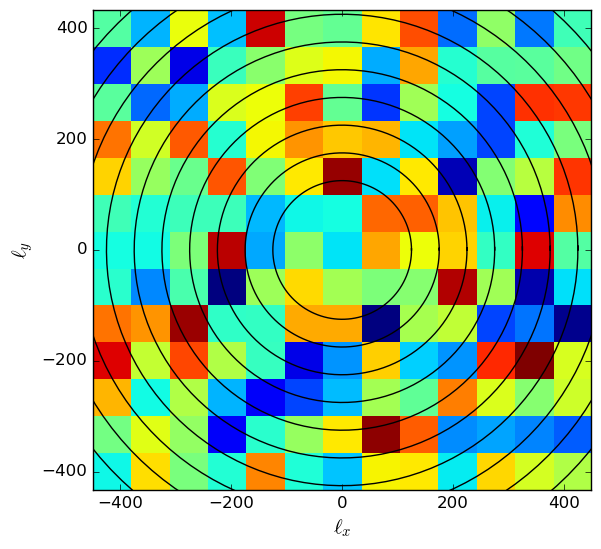
\includegraphics[width=0.5\columnwidth]{p2d.png}
  \caption{Bin in annuli for the Flat Sky power spectrum estimation, we compute the norm $|\bm{\ell}|$ at the center of the Fourier pixel, if the norm is within  $\ell^{\rm min}_{b} \leq |{\bm{\ell}| \leq \ell^{\rm max}_{b}}$  the mode belong to the bin b. (Here I use white noise for the power spectrum value to make the pixels easily distinguishable)}
  \label{fig:p2dbin}
\end{figure}



Where we have introduced $\rho(\bm{\ell})$ which is an arbitrary weight function that can be used to give different weight to different modes (it can be the k-mask, or an azimuthal weight).
Our final estimate for the power spectrum is then
\ba
\hat{C}_{b}= (M_{b, b'})^{-1} \tilde{C}_{b'} 
\ea
This estimator is unbiased. Computing and inverting $M_{b, b'}$ is really the name of the game of power spectrum estimation. It is by far the most expensive step in the power spectrum pipeline.

\subsection{Polarization data in the Flat-Sky approximation}

\subsubsection{From Stokes parameters to E and B field}

The polarization field can be written as  a $2\times2$ symmetric, trace free, tensor 
\ba
P_{ab}(\bm{x})= \frac{1}{2}
\begin{pmatrix} 
Q(\bm{x}) & 
U(\bm{x}) \cr
U(\bm{x}) & 
-Q(\bm{x}) \cr
\end{pmatrix} 
\ea
This form ensures that Q and U transform as expected under a coordinate transformation (imagine for example a rotation of your detectors' array by an angle $\phi$).
Any $2\times2$ symmetric, trace free, tensor can be uniquely decomposed in two parts
\ba 
\eop_{ab} A=(-\partial_{a}\partial_{b}+ \frac{1}{2}\delta_{ab} \nabla^{2})A \ ; \ \bop_{ab}B=\frac{1}{2} (\epsilon_{ac}\partial^{c}\partial_{b} + \epsilon_{bc}\partial^{c}\partial_{a})B
\ea
where A and B are scalar functions. Since the $e^{i\bm{\ell} \bm{x}}$ provide a basis for a scalar function in the plane, we define
\ba
(^{E}e^{i\bm{\ell}\bm{x}})_{ab} &=& N_{\bm{\ell}} \eop_{ab} (e^{i\bm{\ell}\bm{x}})= N_{\bm{\ell}} ( \ell_{a}\ell_{b}- \frac{\bm{\ell}^{2}}{2}\delta_{ab})e^{i\bm{\ell}\bm{x}} \\
(^{B}e^{i\bm{\ell}\bm{x}})_{ab} &=& M_{\bm{\ell}}\bop_{ab} (e^{i\bm{\ell}\bm{x}})=- \frac{M_{\bm{\ell}}}{2} (\epsilon_{ac}\ell^{c}\ell_{b} + \epsilon_{bc}\ell^{c}\ell_{a}) e^{i\bm{\ell}\bm{x}}
\ea
The normalization coefficient $N_{\bm{\ell}}$ is chosen in order to ensure the orthogonality relation.
\ba
\int d^{2}x (^{E}e^{i\bm{\ell}\bm{x}})^{*}_{ab} (^{E}e^{i\bm{\ell}'\bm{x}})^ {ab} = \delta( \bm{\ell}-\bm{\ell}')
\ea
we can expand the polarization field on this basis
\ba
P_{ab}(\bm{x}) &=& \frac{1}{\sqrt{2}} \int d\bm{\ell} E(\bm{\ell}) (^{E}e^{i\bm{\ell}\bm{x}})_{ab} +B({\bm{\ell}}) (^{B}e^{i\bm{\ell}\bm{x}})_{ab} \\
 E({\bm{\ell}}) &=& \frac{2}{\ell^{2}} \int d^{2}x   P_{ab}(\bm{x})   \eop^{ab}(e^{-i\bm{\ell}\bm{x}}) \\
 B({\bm{\ell}}) &=& \frac{2}{\ell^{2}} \int d^{2}x   P_{ab}(\bm{x})  \bop^{ab}(e^{-i\bm{\ell}\bm{x}}) 
\ea
this is equivalent to the spin formalism for polarization data
\ba
E({\bm{\ell}}) &=& Q(\bm{\ell}) \cos 2\phi_{\bm{\ell}}+U(\bm{\ell})\sin 2\phi_{\bm{\ell}}   \\
B({\bm{\ell}}) &=& -Q(\bm{\ell})\sin 2\phi_{\bm{\ell}} +U(\bm{\ell}) \cos 2\phi_{\bm{\ell}}  \\
E({\bm{\ell}}) \pm i B({\bm{\ell}})&=& e^{\mp 2i\phi_{\bm{\ell}}}(Q(\bm{\ell}) \pm i U(\bm{\ell}))
\ea
The Q and U maps geometry can also be read trivially from this set of equation, using a polarisation convention compatible with the output of the map maker, we have

\newcommand{\costwo}{\ensuremath{%
  \mathchoice{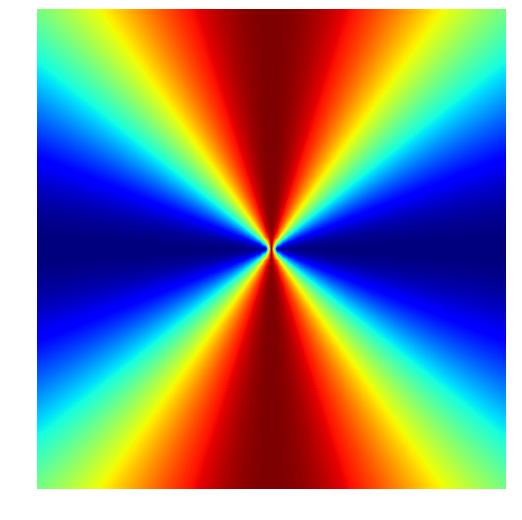
\includegraphics[height=6ex]{cos2.png}}
    {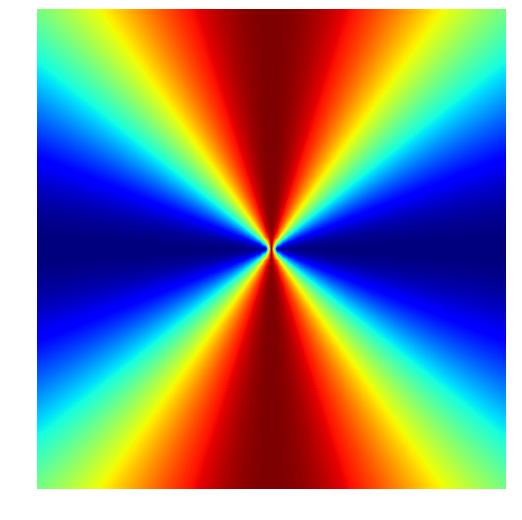
\includegraphics[height=2ex]{cos2.png}}
    {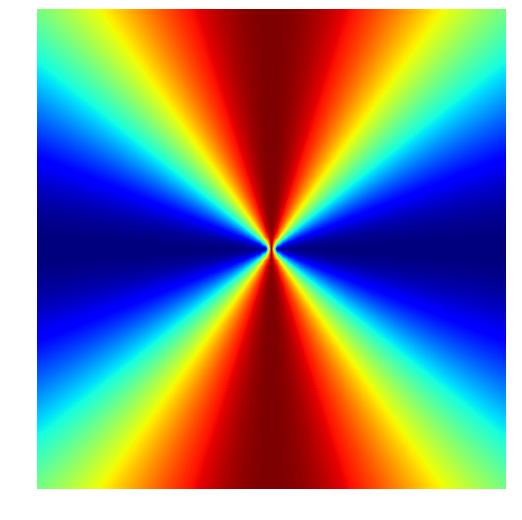
\includegraphics[height=1.5ex]{cos2.png}}
    {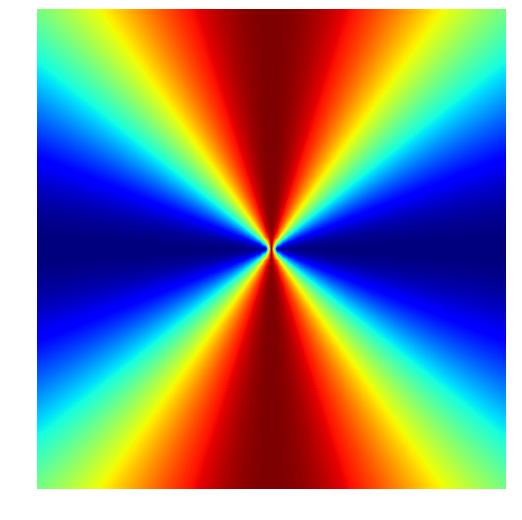
\includegraphics[height=1ex]{cos2.png}}
}}

\newcommand{\sintwo}{\ensuremath{%
  \mathchoice{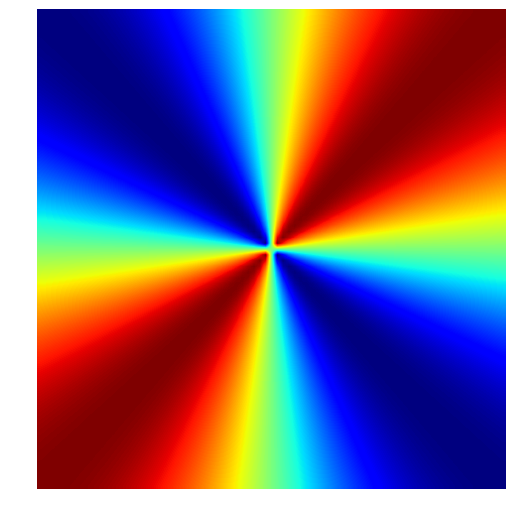
\includegraphics[height=6ex]{sin2.png}}
    {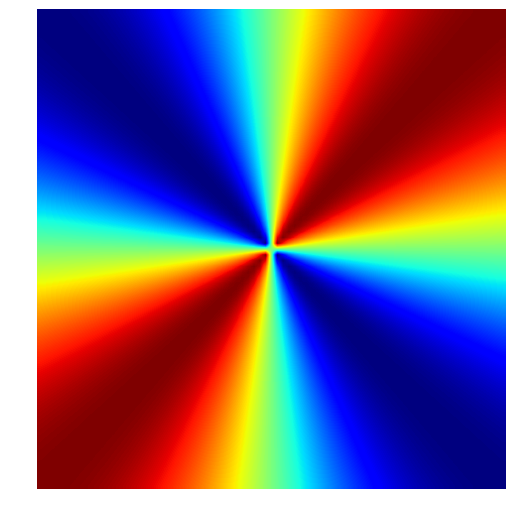
\includegraphics[height=2ex]{sin2.png}}
    {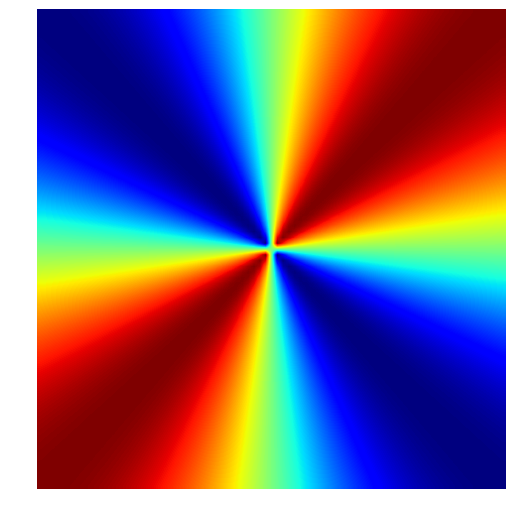
\includegraphics[height=1.5ex]{sin2.png}}
    {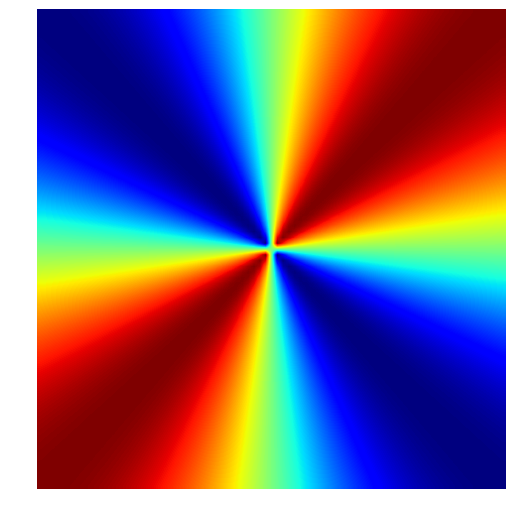
\includegraphics[height=1ex]{sin2.png}}
}}
\ba
Q(\bm{\ell}) &=& E(\bm{\ell}) \costwo - B(\bm{\ell}) \sintwo \\
U(\bm{\ell}) &=& E(\bm{\ell}) \sintwo + B(\bm{\ell}) \costwo
\ea
where we replace the cos and sin by a graphical representation. We can see that if the map is dominated by E modes  Q will have a '+' geometry and U will have a '$\times$' geometry (remember that E and B are isotropic)

\subsubsection{Mode coupling calculation }
We need to extend the mode coupling calculation presented in  \ref{subsec:PSbasis}, to polarization data.  We start by computing the Fourier transform of the Stokes component
\ba
\tilde{Q}_{i}(\bm{\ell}) &=& \int d\bm{\ell'} W (\bm{\ell}-\bm{\ell'}) \left[ b(\bm{\ell'}) Q(\bm{\ell'}) + n^{Q}_{i}(\bm{\ell'})\right]  \\
\tilde{U}_{i}(\bm{\ell}) &=& \int d\bm{\ell'} W (\bm{\ell}-\bm{\ell'}) \left[ b(\bm{\ell'}) U(\bm{\ell'}) + n^{U}_{i}(\bm{\ell'})\right] 
\ea
to simplify the equations and with no loss of generality we will ignore the noise term in the derivation. The observed E and B modes can be written
\ba
\tilde{E}({\bm{\ell}}) \pm i \tilde{B}({\bm{\ell}})&=& e^{\mp 2i\phi_{\bm{\ell}}}(\tilde{Q}(\bm{\ell}) \pm i \tilde{U}(\bm{\ell})) \\
&=& \int d\bm{\ell'} b(\bm{\ell'}) W(\bm{\ell}-\bm{\ell'})  [E({\bm{\ell}'}) \pm i B({\bm{\ell}'})]  e^{  \pm 2i (\phi_{\bm{\ell'}} - \phi_{\bm{\ell}})  }  
\ea
The estimated E (B) modes are then given by a mixture of E and B modes
\ba
\tilde{E}({\bm{\ell}})&=&  \int d\bm{\ell'} b(\bm{\ell'}) W(\bm{\ell}-\bm{\ell'})  [  E({\bm{\ell}'}) \cos  2(\phi_{\bm{\ell'}} - \phi_{\bm{\ell}})  - B({\bm{\ell}'}) \sin  2(\phi_{\bm{\ell'}} - \phi_{\bm{\ell}})  ]   \nonumber \\
\tilde{B}({\bm{\ell}}) &=&  \int d\bm{\ell'} b(\bm{\ell'}) W(\bm{\ell}-\bm{\ell'})  [  E({\bm{\ell}'}) \sin  2(\phi_{\bm{\ell'}} - \phi_{\bm{\ell}})  + B({\bm{\ell}'}) \cos  2(\phi_{\bm{\ell'}} - \phi_{\bm{\ell}})  ]   \nonumber \\
\ea
This is important. The amount of B modes in the map is much smaller than the amount of E modes. The observed B modes map will therefore be dominated by the leakage of E modes due to the window function (the partial sky coverage).
Following what we have done in \ref{subsec:PSbasis}, we can relate the estimated power spectrum to the unbiased power spectrum using a mode coupling matrix
\ba
 \begin{pmatrix}  \tilde{C}_{TE}({\bm{\ell}})\cr \tilde{C}_{TB}({\bm{\ell}})\cr \tilde{C}_{EE} ({\bm{\ell}})  \cr \tilde{C}_{EB} ({\bm{\ell}})  \cr \tilde{C}_{BB} ({\bm{\ell}}) \end{pmatrix} = \sum_{\bm{\ell'} }M_{\bm{\ell}, \bm{\ell'}}\begin{pmatrix}  C_{TE}({\bm{\ell}'})\cr C_{TB}({\bm{\ell}'})\cr C_{EE}({\bm{\ell}'})\cr C_{EB}({\bm{\ell}'})\cr C_{BB}({\bm{\ell}'})\cr  \end{pmatrix} 
\ea
\ba
M_{\bm{\ell}, \bm{\ell'}}= b^{2}(\bm{\ell'})  | W(\bm{\ell}-\bm{\ell'})|^{2} 
\begin{pmatrix} 
\cos \Delta_{\bm{\ell},\bm{\ell'}}  & 
-\sin \Delta_{\bm{\ell},\bm{\ell'}} &
0 & 
0 & 
0 & 
\cr
\sin \Delta_{\bm{\ell},\bm{\ell'}}  & 
\cos \Delta_{\bm{\ell},\bm{\ell'}}  &
0 & 
0 & 
0 & 
  \cr
0 & 
0 &
\cos^{2} \Delta_{\bm{\ell},\bm{\ell'}} & 
-2 \cos \Delta_{\bm{\ell},\bm{\ell'}}  \sin \Delta_{\bm{\ell},\bm{\ell'}} &
\sin^{2} \Delta_{\bm{\ell},\bm{\ell'}}  &  
 \cr
0 & 
0 &
\cos \Delta_{\bm{\ell},\bm{\ell'}}  \sin \Delta_{\bm{\ell},\bm{\ell'}} & 
\cos^{2} \Delta_{\bm{\ell},\bm{\ell'}}-\sin^{2} \Delta_{\bm{\ell},\bm{\ell'}} & 
-\cos \Delta_{\bm{\ell},\bm{\ell'}}  \sin \Delta_{\bm{\ell},\bm{\ell'}} & 
\cr
0 & 
0 &
\sin^{2} \Delta_{\bm{\ell},\bm{\ell'}}  & 
2 \cos \Delta_{\bm{\ell},\bm{\ell'}}  \sin \Delta_{\bm{\ell},\bm{\ell'}} & 
\cos^{2} \Delta_{\bm{\ell},\bm{\ell'}}  & 
\cr
\end{pmatrix}
\ea
With  $\Delta_{\bm{\ell},\bm{\ell'}}= 2(\phi_{\bm{\ell'}} - \phi_{\bm{\ell}})$. Again this matrix can not be inverted. Both the mode coupling matrix and the spectra need to be binned first.

\subsection{Flat sky vs Full sky}

\subsubsection{Full sky power spectrum estimation and the problem with azimuthal weighting}

Similar derivations can be done in the context of full sky power estimation. The math are slighty more complicated as they involve spherical harmonic $Y_{\ell m} (\bm{\hat{n}})$ instead of Fourier modes $e^{i\bm{\ell}\bm{x}}$. It is still interesting to derive the mode coupling matrix for the temperature case, because it will shed light on an important difference between the flat sky and the full sky pipeline. Let's start with the decomposition of the temperature map in spherical harmonic (in practice, we use the python wrapper of the {\it sharp} module which is included in the {\it enlib} library and allow for doing spherical harmonic transform on CAR pixellisation) 
\ba
T(\hat{n}) &=& \sum_{\ell m} a_{\ell m} Y_{\ell m}(\hat{n}) \\
a_{\ell m} &=& \int d \hat{n} T(\hat{n})  Y^{*}_{\ell m}(\hat{n})
\ea
In practice we need to include the effect of a window function
\ba
\tilde{a}_{\ell m} &=& \int d \hat{n} T(\hat{n}) W(\hat{n}) Y^{*}_{\ell m}(\hat{n}) \\
\tilde{a}_{\ell m} &=& \sum_{\ell' m'} a_{\ell' m'} \int d \hat{n} Y_{\ell' m'}(\hat{n}) W(\hat{n}) Y^{*}_{\ell m}(\hat{n}) \\
\tilde{a}_{\ell m} &=& \sum_{\ell' m'} K_{\ell,m, \ell', m'} a_{\ell' m'} 
\ea
similarly to the flat sky case, the effect of the window function is to couple otherwise independent modes $a_{\ell m} $, and the difficulty is to compute the coupling Kernel
\ba
K_{\ell_1,m_1, \ell_2, m_2} &=& \int d \hat{n} Y^{*}_{\ell_1 m_1}(\hat{n}) W(\hat{n}) Y_{\ell_2 m_2}(\hat{n}) \\
&=& \sum_{ \ell_3, m_3} w_{ \ell_3, m_3}  \int d \hat{n} Y^{*}_{\ell_1 m_1}(\hat{n}) Y_{\ell_3 m_3} (\hat{n}) Y_{\ell_2 m_2}(\hat{n})
\ea
This integral can be express in term of Wigner 3j symbol (they are usually introduced in the context of the addition of angular momentum in Quantum mechanics).
 \ba
\int d \hat{n} Y^{*}_{\ell_1 m_1}(\hat{n}) Y_{\ell_3 m_3} (\hat{n}) Y_{\ell_2 m_2}(\hat{n}) &=& (-1)^{m_1} \left[\frac{(2\ell_1+1) (2\ell_2+1) (2\ell_3+1)}{4\pi} \right]^{1/2} \\ \nonumber
&\times& \left(\begin{array}{clcr}
\ell_1 & \ell_2 & \ell_3\\
0 & 0 & 0 \end{array}\right)
\left(\begin{array}{clcr}
\ell_1 & \ell_2 & \ell_3\\
-m_{1} & m_{2} & m_{3} \end{array}\right)
\ea
One nice thing about Wigner 3j is the following property
\ba
\sum_{m_1 m_2}
\left(\begin{array}{clcr}
\ell_1 & \ell_2 & \ell_3\\
m_{1} & m_{2} & m_{3} \end{array}\right)
\left(\begin{array}{clcr}
\ell_1 & \ell_2 & \ell^{'}_3\\
m_{1} & m_{2} & m^{'}_{3} \end{array}\right)= \delta_{m_3 m^{'}_3} \delta_{\ell_3 \ell^{'}_3} \delta(\ell_1, \ell_2, \ell_3) \frac{1}{2\ell_3+1}
\ea
The mean of our estimator for the power spectrum is given by
\ba
\langle \tilde{C}_{\ell} \rangle &=& \frac{1}{2\ell +1}\sum^{\ell}_{m=-\ell} \langle \tilde{a}_{\ell m} \tilde{a}^{*}_{\ell m} \rangle \\
&=&  \frac{1}{2\ell +1}\sum^{\ell}_{m=-\ell} \langle \sum_{\ell_1 m_1} K_{\ell,m, \ell_1, m_1} a_{\ell_1 m_1}  \sum_{\ell_2 m_2} K^{*}_{\ell,m, \ell_2, m_2} a^{*}_{\ell_2 m_2} \rangle \\
&=&  \frac{1}{2\ell +1}\sum^{\ell}_{m=-\ell}  \sum_{\ell_1 m_1} \langle C_{\ell_1} \rangle | K_{\ell,m, \ell_1, m_1} |^{2} 
\ea
The next move is to expand and simplify the Kernel
\ba
\langle \tilde{C}_{\ell} \rangle &=&    \sum_{\ell_1}  \frac{2\ell_1 +1}{4\pi} \langle C_{\ell_1} \rangle  \sum_{ \ell_3, m_3} w_{ \ell_3, m_3}  \sum_{ \ell_4, m_4} w^{*}_{ \ell_4, m_4}  (2\ell_3+1)^{1/2} (2\ell_4+1)^{1/2} \label{eq:line1mcm} \\ \nonumber 
&\times &
\left(\begin{array}{clcr}
\ell & \ell_1 & \ell_3\\
0 & 0 & 0 \end{array}\right)
\left(\begin{array}{clcr}
\ell & \ell_1 & \ell_4\\
0 & 0 & 0 \end{array}\right)
\sum_{m,m_1}
\left(\begin{array}{clcr}
\ell & \ell_1 & \ell_3\\
-m & m_{1} & m_{3} \end{array}\right)
\left(\begin{array}{clcr}
\ell & \ell_1 & \ell_4\\
-m & m_{1} & m_{4} \end{array}\right) \\
&=&    \sum_{\ell_1}  \frac{2\ell_1 +1}{4\pi} \langle C_{\ell_1} \rangle  \sum_{ \ell_3, m_3} w_{ \ell_3, m_3}  \sum_{ \ell_4, m_4} w^{*}_{ \ell_4, m_4}  (2\ell_3+1)^{1/2} (2\ell_4+1)^{1/2} \label{eq:line2mcm} \\ \nonumber 
&\times &
\left(\begin{array}{clcr}
\ell & \ell_1 & \ell_3\\
0 & 0 & 0 \end{array}\right)
\left(\begin{array}{clcr}
\ell & \ell_1 & \ell_4\\
0 & 0 & 0 \end{array}\right)
\delta_{m_3 m_4} \delta_{\ell_3 \ell_4} \delta(\ell_1, \ell_2, \ell_3) \frac{1}{2\ell_3+1} \\
&=&    \sum_{\ell_1}  \frac{2\ell_1 +1}{4\pi} \langle C_{\ell_1} \rangle  \sum_{ \ell_3, m_3} w_{ \ell_3, m_3}   w^{*}_{ \ell_3, m_3}    
\left(\begin{array}{clcr}
\ell & \ell_1 & \ell_3\\
0 & 0 & 0 \end{array}\right)^{2} \\
&=&    \sum_{\ell_1}  \frac{2\ell_1 +1}{4\pi} \langle C_{\ell_1} \rangle  \sum_{ \ell_3} (2\ell_3+1) {\cal W}_{\ell_3} 
\left(\begin{array}{clcr}
\ell & \ell_1 & \ell_3\\
0 & 0 & 0 \end{array}\right)^{2} \\
&=& \sum_{\ell_1}M_{ \ell, \ell_1} \langle C_{\ell_1} \rangle
\ea
At the end, the expression of the mode coupling is simple  
\ba
M_{ \ell, \ell_1}=   \frac{2\ell_1 +1}{4\pi}  \sum_{ \ell_3} (2\ell_3+1) {\cal W}_{\ell_3} 
\left(\begin{array}{clcr}
\ell & \ell_1 & \ell_3\\
0 & 0 & 0 \end{array}\right)^{2}
\ea
There is an important difference between this formalism and the one of the Flat Sky approximation. The simplification between Eq \ref{eq:line1mcm} and Eq \ref{eq:line2mcm} allows us to reduce the computation time drastically. However, imagine that instead of using the estimator
\ba
 \tilde{C}_{\ell}  &=& \frac{1}{2\ell +1}\sum^{\ell}_{m=-\ell}  \tilde{a}_{\ell m} \tilde{a}^{*}_{\ell m}  
\ea
We would like to switch to an estimator allowing for different weighting of the harmonic coefficients
\ba
 \tilde{C}_{\ell}  &=& \frac{1}{2\ell +1}\sum^{\ell}_{m=-\ell} \rho_{\ell m}  \tilde{a}_{\ell m} \tilde{a}^{*}_{\ell m}  
\ea
In that case the last term of equation Eq \ref{eq:line1mcm} becomes
\ba
\sum_{m,m_1} \rho_{\ell m}
\left(\begin{array}{clcr}
\ell & \ell_1 & \ell_3\\
-m & m_{1} & m_{3} \end{array}\right)
\left(\begin{array}{clcr}
\ell & \ell_1 & \ell_4\\
-m & m_{1} & m_{4} \end{array}\right)
\ea
preventing the important simplication. In the Flat-Sky case, we can afford to compute the mode coupling exactly and include the effect of k-mask and azimuthal weighting in a straightforward way. For the full sky case, we are applying the k-mask on data and deconvolve its effect using a transfer function.  \\

Let's now move on to the polarisation case, the polarisation field ${}_{\pm 2} P(\hat{n})= (Q \pm iU)(\hat{n})$ can be decomposed into E and B modes
\ba
{}_{\pm 2} P(\hat{n}) = - \sum_{\ell m} (a^{E}_{\ell m} \pm i a^{B}_{\ell m}) {}_{\pm 2} Y_{\ell m} (\hat{n})
\ea
where ${}_{\pm 2} Y_{\ell m} (\hat{n})$ are spin-2 spherical harmonics.
We can express E and B modes as a function of P
 \ba
 a^{E}_{\ell m}&=& -\frac{1}{2}  \int \left(  {}_{2} P(\hat{n})  {}_{2} Y^{*}_{\ell m} (\hat{n})+  {}_{-2} P(\hat{n})  {}_{-2} Y^{*}_{\ell m} (\hat{n}) \right) d\hat{n} \\
 a^{B}_{\ell m}&=& \frac{i}{2}  \int \left(  {}_{2} P(\hat{n})  {}_{2} Y^{*}_{\ell m} (\hat{n})-  {}_{-2} P(\hat{n})  {}_{-2} Y^{*}_{\ell m} (\hat{n}) \right) d\hat{n}
 \ea
 or simply
 \ba
  a^{E}_{\ell m} \pm i a^{B}_{\ell m} = - \int {}_{\pm 2} P(\hat{n}) {}_{\pm 2} Y^{*}_{\ell m} (\hat{n})d\hat{n}
 \ea
including a window function we get
 \ba
  \tilde{a}^{E}_{\ell m} \pm i \tilde{a}^{B}_{\ell m} = - \int W(\hat{n}) {}_{\pm 2} P(\hat{n}) {}_{\pm 2} Y^{*}_{\ell m} (\hat{n})d\hat{n}
 \ea
 re-expending ${}_{\pm 2} P(\hat{n})$ in spherical harmonic
 \ba
   \tilde{a}^{E}_{\ell m} \pm i   \tilde{a}^{B}_{\ell m} =  \sum_{\ell' m'} (a^{E}_{\ell' m'} \pm i a^{B}_{\ell' m'}) \int W(\hat{n}) {}_{\pm 2} Y_{\ell' m'} (\hat{n})  {}_{\pm 2} Y^{*}_{\ell m} (\hat{n})d\hat{n}
 \ea
Then
\ba
   \tilde{a}^{E}_{\ell m} &= & \frac{1}{2} \sum_{\ell' m'} a^{E}_{\ell' m'} \left[ \int W(\hat{n}) {}_{ 2} Y_{\ell' m'} (\hat{n})  {}_{ 2} Y^{*}_{\ell m} (\hat{n})d\hat{n} + \int W(\hat{n}) {}_{ -2} Y_{\ell' m'} (\hat{n})  {}_{ -2} Y^{*}_{\ell m} (\hat{n})d\hat{n} \right] \\
 &+& \frac{i}{2} \sum_{\ell' m'}  a^{B}_{\ell' m'} \left[ \int W(\hat{n}) {}_{ 2} Y_{\ell' m'} (\hat{n})  {}_{ 2} Y^{*}_{\ell m} (\hat{n})d\hat{n} -\int W(\hat{n}) {}_{ -2} Y_{\ell' m'} (\hat{n})  {}_{ -2} Y^{*}_{\ell m} (\hat{n})d\hat{n}\right] \\ 
 &=&  \sum_{\ell' m'} K^{\rm diag}_{\ell m, \ell' m'} a^{E}_{\ell' m'} + i K^{\rm off}_{\ell m, \ell' m'} a^{B}_{\ell' m'}
\ea
and 

\ba
   \tilde{a}^{B}_{\ell m} &= & \frac{-i}{2} \sum_{\ell' m'} a^{E}_{\ell' m'} \left[ \int W(\hat{n}) {}_{ 2} Y_{\ell' m'} (\hat{n})  {}_{ 2} Y^{*}_{\ell m} (\hat{n})d\hat{n} - \int W(\hat{n}) {}_{ -2} Y_{\ell' m'} (\hat{n})  {}_{ -2} Y^{*}_{\ell m} (\hat{n})d\hat{n} \right] \\
 &+& \frac{1}{2} \sum_{\ell' m'}  a^{B}_{\ell' m'} \left[ \int W(\hat{n}) {}_{ 2} Y_{\ell' m'} (\hat{n})  {}_{ 2} Y^{*}_{\ell m} (\hat{n})d\hat{n} +\int W(\hat{n}) {}_{ -2} Y_{\ell' m'} (\hat{n})  {}_{ -2} Y^{*}_{\ell m} (\hat{n})d\hat{n}\right] \\
 &=&  \sum_{\ell' m'} -i K^{\rm off}_{\ell m, \ell' m'} a^{E}_{\ell' m'} + K^{\rm diag}_{\ell m, \ell' m'} a^{B}_{\ell' m'}
\ea

Following a similar derivation than the one presented for the flat sky case, we can obtain the full expression for the mode coupling matrix in the full sky case: 
\ba
 \begin{pmatrix}  \tilde{C}_{TT}(\ell) \cr \tilde{C}_{TE}(\ell)\cr \tilde{C}_{TB}(\ell)\cr \tilde{C}_{EE}(\ell)\cr \tilde{C}_{EB}(\ell)\cr \tilde{C}_{BB}(\ell)\cr \end{pmatrix} = \sum_{\ell'} M_{\ell, \ell'} 
  \begin{pmatrix}  C_{TT}(\ell') \cr C_{TE}(\ell)\cr C_{TB}(\ell')\cr C_{EE}(\ell')\cr C_{EB}(\ell')\cr C_{BB}(\ell')\cr \end{pmatrix}
\ea
with
\ba
M_{\ell, \ell'}=   
\begin{pmatrix} 
M_{TTTT} &
0 & 
0 &
0 & 
0 & 
0 & 
\cr
0 & 
M_{TETE} & 
0 &
0 & 
0 & 
0 & 
\cr
0 &
0 & 
M_{TBTB} & 
0 & 
0 & 
0 & 
  \cr
0 &
0 & 
0 &
M_{EEEE}& 
0 &
M_{EEBB} &  
 \cr
0 &
0 & 
0 &
0 & 
M_{EBEB}  &
0&  
\cr
0 &
0 & 
0 &
M_{BBEE} & 
0  &
M_{BBBB}&  
\cr
\end{pmatrix}
\ea
with elements
\ba
M^{TTTT}_{\ell \ell'}&=&  \frac{2\ell'+1}{4\pi} B^{2}_{\ell'} \sum_{\ell''} (2\ell''+1) {\cal W}^{TT}_{\ell''}    
\left(\begin{array}{clcr}
\ell & \ell' & \ell''\\
0 & 0 & 0 \end{array}\right)^{2}
 \nonumber \\
M^{TETE}_{\ell \ell'}&=& M^{TBTB}_{\ell \ell'}= \frac{2\ell'+1}{4\pi}B^{2}_{\ell'}\sum_{\ell''} (2\ell''+1) {\cal W}^{PT}_{\ell''}    
\left(\begin{array}{clcr}
\ell & \ell' & \ell''\\
0 & 0 & 0 \end{array}\right)
\left(\begin{array}{clcr}
\ell & \ell' & \ell''\\
2 & -2 & 0 \end{array}\right) \nonumber \\
M^{EEEE}_{\ell \ell'} &=&M^{BBBB}_{\ell \ell'}=  \frac{2\ell'+1}{4\pi} B^{2}_{\ell'} \sum_{\ell''} (2\ell''+1) {\cal W}^{P}_{\ell''}
\left(\begin{array}{clcr}
\ell & \ell' & \ell''\\
2 & -2 & 0 \end{array}\right)^{2}
\frac{1 + (-1)^{\ell+ \ell' + \ell''}}{2} \nonumber \\
M^{EEBB}_{\ell \ell'} &=&M^{BBEE}_{\ell \ell'}=  \frac{2\ell'+1}{4\pi} B^{2}_{\ell'} \sum_{\ell''} (2\ell''+1) {\cal W}^{P}_{\ell''}
\left(\begin{array}{clcr}
\ell & \ell' & \ell''\\
2 & -2 & 0 \end{array}\right)^{2}
\frac{1 - (-1)^{\ell+ \ell' + \ell''}}{2} \nonumber \\
M^{EBEB}_{\ell \ell'}&=& M^{EEEE}_{\ell \ell'}-M^{EEBB}_{\ell \ell'} 
\ea

\subsubsection{Comparaison between full sky and flat sky power spectra}


\subsection{Azimuthal weighting}

\subsection{Prewithening/ Mask apodization}

\subsection{Cross frequencies and Cross seasons  power spectra}

\subsection{Planck calibration}

\subsection{Covariance matrix}


%An estimator of the two dimensional cross power spectrum is obtained by taking the average of each cross spectrum
%\ba
%\tilde{C}(\bm{\ell}) &=& \frac{1}{N_c}\sum_{i,k>i} \tilde{T}_{i}(\bm{\ell}) \tilde{T}_{k}(\bm{\ell}) \\
%N_c &=& \sum_{i,k>i} 1=  N_{s}(N_{s}+1)/2
%\ea
%Let us focus on a given pair of split 
 
\section{Lensing}

\subsection{Data prep}
\subsection{Sims}
\subsection{Kappa maps}
\subsection{Biases and Power spectra}
\subsection{Delensing}
\subsection{Likelihood}

For any T, E, B pair that we denote as $x$, the quadratic estimator starts off being wrong by some cosmology-dependent normalization (all $LM$ indices are suppressed),

$$
\langle \hat{x} \rangle = R_{x} \kappa_x 
$$

We correct by some fiducial cosmology letting the estimator be $\hat{\kappa}_x = \hat{x} / R^0_x$. This means the expected value is now,

$$
\langle\hat\kappa\rangle = \frac{R_x}{R^0_x}\kappa 
$$

Next, we calculate the power spectrum, but correct for the anticipated $N_1$ bias,

$$
\hat{C}_{xy}=\frac{1}{R^0_xR^0_y}\hat{x}\hat{y} - N_{1,xy}^0
$$

which leads to an expected theory power spectrum of,

$$
C_{xy}^{\mathrm{th}}=\frac{R_xR_y}{R^0_xR^0_y}C_{xy} + N_{1,xy} - N_{1,xy}^0
$$

Expanding the $R$'s and $N$'s about the fiducial by some parametrization $\boldsymbol{\theta}$,

\newcommand{\bth}{\boldsymbol{\theta}}
\newcommand{\bna}{\boldsymbol{\nabla}}

\begin{align*}
C_{xy}^{\mathrm{th}}&\approx\frac{R^0_xR^0_y+\bna^0_{\bth} (R_xR_y)\cdot (\bth-\bth_0)}{R^0_xR^0_y}C_{xy} + \bna^0_{\bth} N_{1,xy}\cdot (\bth-\bth_0) \\
&\approx C_{xy}+\bna^0_{\bth} \mathrm{ln}(R_xR_y)\cdot (\bth-\bth_0)C_{xy} + \bna^0_{\bth} N_{1,xy}\cdot (\bth-\bth_0)
\end{align*}

The Planck parametrization is $\bth=\{C_x, C_{xy}\}$ (the CMB and convergence spectra, respectively).

\subsubsection{Corrections}

\newcommand{\bell}{\boldsymbol{\ell}}
\newcommand{\bL}{\boldsymbol{L}}

For each polcomb in $\alpha=\{\mathrm{TT,TE,EE,EB}\}$, we calculate the normalization

$$
L^2A_{\alpha}^{-1}(\bL) = \int \frac{d^2\bell_1}{(2\pi)^2} f_{\alpha}(\bell_1,\bell_2)F_{\alpha}^0(\bell_1,\bell_2)
$$

Here, $F_{\alpha}^0(\bell_1,\bell_2)$ and $f_{\alpha}(\bell_1,\bell_2)$ are functions of the CMB power spectra. The former is always evaluated at the fiducial cosmology assumed in the main analysis. We calculate derivatives of the normalization with respect to CMB power spectra by shifting the amplitude in annuli of width $\Delta \ell$ of the respective 2D CMB power spectra that are used in $f_{\alpha}(\bell_1,\bell_2)$. For the TT case,

$$
R(\bL) \equiv L^2A_{TT}^{-1}(\bL) = \int \frac{d^2\bell_1}{(2\pi)^2} (C_{\ell_1}(\bL.\bell_1)+C_{\ell_2}(\bL.\bell_2))F_{TT}^0(\bell_1,\bell_2)
$$

$$
\frac{\partial R(\bL)}{\partial C_{\ell}} = \int \frac{d^2\bell_1}{(2\pi)^2} (\delta(\ell_1-\ell)(\bL.\bell_1)+(\delta(\ell_2-\ell)(\bL.\bell_2))F_{TT}^0(\bell_1,\bell_2)
$$

$$
\frac{\partial^2 R(\bL)}{\partial C^2_{\ell}} = 0
$$

Ignoring the N1 correction for now, we expand up to all orders in the product of $R$s, which only gives one additional term.

\begin{align*}
C_{xy}^{\mathrm{th}}&\approx\frac{R^0_xR^0_y+\bna_{\bth} (R_xR_y)\cdot (\bth-\bth_0)+\bna^2_{\bth} (R_xR_y)\cdot (\bth-\bth_0)^2}{R^0_xR^0_y}C_{xy}  \\
&\approx C_{xy}+\bna^0_{\bth} \mathrm{ln}(R_xR_y)\cdot (\bth-\bth_0)C_{xy} +2\bna^0_{\bth} \mathrm{ln}R_x\bna^0_{\bth}\mathrm{ln}R_y\cdot (\bth-\bth_0)^2C_{xy} 
\end{align*}

Note that the $C_{xy}$ here is evaluated at the point in the chain, rather than at the fiducial. Unlike the Planck corrections, the difference between the two does matter here since we need to be correct up to all orders.

\subsection{Cluster lensing}

\section{Foregrounds }


\section{Cosmological Parameters }


\end{document}


